% Options for packages loaded elsewhere
\PassOptionsToPackage{unicode}{hyperref}
\PassOptionsToPackage{hyphens}{url}
%
\documentclass[
]{article}
\usepackage{amsmath,amssymb}
\usepackage{iftex}
\ifPDFTeX
  \usepackage[T1]{fontenc}
  \usepackage[utf8]{inputenc}
  \usepackage{textcomp} % provide euro and other symbols
\else % if luatex or xetex
  \usepackage{unicode-math} % this also loads fontspec
  \defaultfontfeatures{Scale=MatchLowercase}
  \defaultfontfeatures[\rmfamily]{Ligatures=TeX,Scale=1}
\fi
\usepackage{lmodern}
\ifPDFTeX\else
  % xetex/luatex font selection
\fi
% Use upquote if available, for straight quotes in verbatim environments
\IfFileExists{upquote.sty}{\usepackage{upquote}}{}
\IfFileExists{microtype.sty}{% use microtype if available
  \usepackage[]{microtype}
  \UseMicrotypeSet[protrusion]{basicmath} % disable protrusion for tt fonts
}{}
\makeatletter
\@ifundefined{KOMAClassName}{% if non-KOMA class
  \IfFileExists{parskip.sty}{%
    \usepackage{parskip}
  }{% else
    \setlength{\parindent}{0pt}
    \setlength{\parskip}{6pt plus 2pt minus 1pt}}
}{% if KOMA class
  \KOMAoptions{parskip=half}}
\makeatother
\usepackage{xcolor}
\usepackage[margin=1in]{geometry}
\usepackage{color}
\usepackage{fancyvrb}
\newcommand{\VerbBar}{|}
\newcommand{\VERB}{\Verb[commandchars=\\\{\}]}
\DefineVerbatimEnvironment{Highlighting}{Verbatim}{commandchars=\\\{\}}
% Add ',fontsize=\small' for more characters per line
\usepackage{framed}
\definecolor{shadecolor}{RGB}{248,248,248}
\newenvironment{Shaded}{\begin{snugshade}}{\end{snugshade}}
\newcommand{\AlertTok}[1]{\textcolor[rgb]{0.94,0.16,0.16}{#1}}
\newcommand{\AnnotationTok}[1]{\textcolor[rgb]{0.56,0.35,0.01}{\textbf{\textit{#1}}}}
\newcommand{\AttributeTok}[1]{\textcolor[rgb]{0.13,0.29,0.53}{#1}}
\newcommand{\BaseNTok}[1]{\textcolor[rgb]{0.00,0.00,0.81}{#1}}
\newcommand{\BuiltInTok}[1]{#1}
\newcommand{\CharTok}[1]{\textcolor[rgb]{0.31,0.60,0.02}{#1}}
\newcommand{\CommentTok}[1]{\textcolor[rgb]{0.56,0.35,0.01}{\textit{#1}}}
\newcommand{\CommentVarTok}[1]{\textcolor[rgb]{0.56,0.35,0.01}{\textbf{\textit{#1}}}}
\newcommand{\ConstantTok}[1]{\textcolor[rgb]{0.56,0.35,0.01}{#1}}
\newcommand{\ControlFlowTok}[1]{\textcolor[rgb]{0.13,0.29,0.53}{\textbf{#1}}}
\newcommand{\DataTypeTok}[1]{\textcolor[rgb]{0.13,0.29,0.53}{#1}}
\newcommand{\DecValTok}[1]{\textcolor[rgb]{0.00,0.00,0.81}{#1}}
\newcommand{\DocumentationTok}[1]{\textcolor[rgb]{0.56,0.35,0.01}{\textbf{\textit{#1}}}}
\newcommand{\ErrorTok}[1]{\textcolor[rgb]{0.64,0.00,0.00}{\textbf{#1}}}
\newcommand{\ExtensionTok}[1]{#1}
\newcommand{\FloatTok}[1]{\textcolor[rgb]{0.00,0.00,0.81}{#1}}
\newcommand{\FunctionTok}[1]{\textcolor[rgb]{0.13,0.29,0.53}{\textbf{#1}}}
\newcommand{\ImportTok}[1]{#1}
\newcommand{\InformationTok}[1]{\textcolor[rgb]{0.56,0.35,0.01}{\textbf{\textit{#1}}}}
\newcommand{\KeywordTok}[1]{\textcolor[rgb]{0.13,0.29,0.53}{\textbf{#1}}}
\newcommand{\NormalTok}[1]{#1}
\newcommand{\OperatorTok}[1]{\textcolor[rgb]{0.81,0.36,0.00}{\textbf{#1}}}
\newcommand{\OtherTok}[1]{\textcolor[rgb]{0.56,0.35,0.01}{#1}}
\newcommand{\PreprocessorTok}[1]{\textcolor[rgb]{0.56,0.35,0.01}{\textit{#1}}}
\newcommand{\RegionMarkerTok}[1]{#1}
\newcommand{\SpecialCharTok}[1]{\textcolor[rgb]{0.81,0.36,0.00}{\textbf{#1}}}
\newcommand{\SpecialStringTok}[1]{\textcolor[rgb]{0.31,0.60,0.02}{#1}}
\newcommand{\StringTok}[1]{\textcolor[rgb]{0.31,0.60,0.02}{#1}}
\newcommand{\VariableTok}[1]{\textcolor[rgb]{0.00,0.00,0.00}{#1}}
\newcommand{\VerbatimStringTok}[1]{\textcolor[rgb]{0.31,0.60,0.02}{#1}}
\newcommand{\WarningTok}[1]{\textcolor[rgb]{0.56,0.35,0.01}{\textbf{\textit{#1}}}}
\usepackage{graphicx}
\makeatletter
\newsavebox\pandoc@box
\newcommand*\pandocbounded[1]{% scales image to fit in text height/width
  \sbox\pandoc@box{#1}%
  \Gscale@div\@tempa{\textheight}{\dimexpr\ht\pandoc@box+\dp\pandoc@box\relax}%
  \Gscale@div\@tempb{\linewidth}{\wd\pandoc@box}%
  \ifdim\@tempb\p@<\@tempa\p@\let\@tempa\@tempb\fi% select the smaller of both
  \ifdim\@tempa\p@<\p@\scalebox{\@tempa}{\usebox\pandoc@box}%
  \else\usebox{\pandoc@box}%
  \fi%
}
% Set default figure placement to htbp
\def\fps@figure{htbp}
\makeatother
\setlength{\emergencystretch}{3em} % prevent overfull lines
\providecommand{\tightlist}{%
  \setlength{\itemsep}{0pt}\setlength{\parskip}{0pt}}
\setcounter{secnumdepth}{-\maxdimen} % remove section numbering
\usepackage{ctex}
\usepackage{bookmark}
\IfFileExists{xurl.sty}{\usepackage{xurl}}{} % add URL line breaks if available
\urlstyle{same}
\hypersetup{
  pdftitle={homework4},
  pdfauthor={zza},
  hidelinks,
  pdfcreator={LaTeX via pandoc}}

\title{homework4}
\author{zza}
\date{2025-07-01}

\begin{document}
\maketitle

\subsection{1}\label{section}

\begin{Shaded}
\begin{Highlighting}[]
\NormalTok{ckm\_nodes }\OtherTok{\textless{}{-}} \FunctionTok{read.csv}\NormalTok{(}\StringTok{\textquotesingle{}ckm\_nodes.csv\textquotesingle{}}\NormalTok{)  }


\NormalTok{noinfor }\OtherTok{\textless{}{-}} \FunctionTok{which}\NormalTok{(}\FunctionTok{is.na}\NormalTok{(ckm\_nodes}\SpecialCharTok{$}\NormalTok{adoption\_date))  }


\NormalTok{ckm\_nodes }\OtherTok{\textless{}{-}}\NormalTok{ ckm\_nodes[}\SpecialCharTok{{-}}\NormalTok{noinfor, ]  }


\NormalTok{ckm\_network }\OtherTok{\textless{}{-}} \FunctionTok{read.table}\NormalTok{(}\StringTok{\textquotesingle{}ckm\_network.dat\textquotesingle{}}\NormalTok{)  }


\NormalTok{ckm\_network }\OtherTok{\textless{}{-}}\NormalTok{ ckm\_network[}\SpecialCharTok{{-}}\NormalTok{noinfor, }\SpecialCharTok{{-}}\NormalTok{noinfor]  }
\end{Highlighting}
\end{Shaded}

\subsection{2}\label{section-1}

\begin{Shaded}
\begin{Highlighting}[]
\NormalTok{num\_doctors }\OtherTok{\textless{}{-}} \FunctionTok{nrow}\NormalTok{(ckm\_nodes)  }

\NormalTok{num\_months }\OtherTok{\textless{}{-}} \DecValTok{17}  


\NormalTok{result\_df }\OtherTok{\textless{}{-}} \FunctionTok{expand.grid}\NormalTok{(}
  \AttributeTok{doctor\_id =} \DecValTok{1}\SpecialCharTok{:}\NormalTok{num\_doctors, }
  \AttributeTok{month =} \DecValTok{1}\SpecialCharTok{:}\NormalTok{num\_months        }
\NormalTok{) }\SpecialCharTok{\%\textgreater{}\%} 

  \FunctionTok{mutate}\NormalTok{(}
    \AttributeTok{started\_this\_month =} \ConstantTok{FALSE}\NormalTok{,        }
    \AttributeTok{already\_started\_before =} \ConstantTok{FALSE}\NormalTok{,    }
    \AttributeTok{contacts\_started\_before =} \DecValTok{0}\NormalTok{,       }
    \AttributeTok{contacts\_started\_by =} \DecValTok{0}            
\NormalTok{  )}


\ControlFlowTok{for}\NormalTok{ (i }\ControlFlowTok{in} \DecValTok{1}\SpecialCharTok{:}\NormalTok{num\_doctors) \{}
\NormalTok{  adoption\_date }\OtherTok{\textless{}{-}}\NormalTok{ ckm\_nodes}\SpecialCharTok{$}\NormalTok{adoption\_date[i]  }
  \ControlFlowTok{for}\NormalTok{ (j }\ControlFlowTok{in} \DecValTok{1}\SpecialCharTok{:}\NormalTok{num\_months) \{}
    \ControlFlowTok{if}\NormalTok{ (}\SpecialCharTok{!}\FunctionTok{is.na}\NormalTok{(adoption\_date)) \{  }
      
\NormalTok{      result\_df[(result\_df}\SpecialCharTok{$}\NormalTok{doctor\_id }\SpecialCharTok{==}\NormalTok{ i) }\SpecialCharTok{\&}\NormalTok{ (result\_df}\SpecialCharTok{$}\NormalTok{month }\SpecialCharTok{==}\NormalTok{ j), }
                \StringTok{"started\_this\_month"}\NormalTok{] }\OtherTok{\textless{}{-}}\NormalTok{ (adoption\_date }\SpecialCharTok{==}\NormalTok{ j)  }
      
\NormalTok{      result\_df[(result\_df}\SpecialCharTok{$}\NormalTok{doctor\_id }\SpecialCharTok{==}\NormalTok{ i) }\SpecialCharTok{\&}\NormalTok{ (result\_df}\SpecialCharTok{$}\NormalTok{month }\SpecialCharTok{==}\NormalTok{ j), }
                \StringTok{"already\_started\_before"}\NormalTok{] }\OtherTok{\textless{}{-}}\NormalTok{ (adoption\_date }\SpecialCharTok{\textless{}}\NormalTok{ j)  }
      

\NormalTok{      contacts\_before }\OtherTok{\textless{}{-}} \FunctionTok{sum}\NormalTok{(ckm\_network[i, ] }\SpecialCharTok{\&}\NormalTok{ ckm\_nodes}\SpecialCharTok{$}\NormalTok{adoption\_date }\SpecialCharTok{\textless{}=}\NormalTok{ j }\SpecialCharTok{{-}} \DecValTok{1}\NormalTok{)  }
\NormalTok{      result\_df[(result\_df}\SpecialCharTok{$}\NormalTok{doctor\_id }\SpecialCharTok{==}\NormalTok{ i) }\SpecialCharTok{\&}\NormalTok{ (result\_df}\SpecialCharTok{$}\NormalTok{month }\SpecialCharTok{==}\NormalTok{ j), }
                \StringTok{"contacts\_started\_before"}\NormalTok{] }\OtherTok{\textless{}{-}}\NormalTok{ contacts\_before}
      
\NormalTok{      contacts\_by }\OtherTok{\textless{}{-}} \FunctionTok{sum}\NormalTok{(ckm\_network[i, ] }\SpecialCharTok{\&}\NormalTok{ ckm\_nodes}\SpecialCharTok{$}\NormalTok{adoption\_date }\SpecialCharTok{\textless{}=}\NormalTok{ j)  }
\NormalTok{      result\_df[(result\_df}\SpecialCharTok{$}\NormalTok{doctor\_id }\SpecialCharTok{==}\NormalTok{ i) }\SpecialCharTok{\&}\NormalTok{ (result\_df}\SpecialCharTok{$}\NormalTok{month }\SpecialCharTok{==}\NormalTok{ j),}
                \StringTok{"contacts\_started\_by"}\NormalTok{] }\OtherTok{\textless{}{-}}\NormalTok{ contacts\_by}
\NormalTok{    \}}
\NormalTok{  \}}
\NormalTok{\}}

\CommentTok{\# 查看结果}
\FunctionTok{dim}\NormalTok{(result\_df)   }
\end{Highlighting}
\end{Shaded}

\begin{verbatim}
## [1] 2125    6
\end{verbatim}

\subsection{3}\label{section-2}

\subsubsection{a}\label{a}

\begin{Shaded}
\begin{Highlighting}[]
\NormalTok{contacts\_per\_doctor }\OtherTok{\textless{}{-}} \FunctionTok{rowSums}\NormalTok{(ckm\_network)}

\NormalTok{max\_contacts }\OtherTok{\textless{}{-}} \FunctionTok{max}\NormalTok{(contacts\_per\_doctor)}
\FunctionTok{cat}\NormalTok{(}\StringTok{"医生的最大社交连接数:"}\NormalTok{, max\_contacts, }\StringTok{"}\SpecialCharTok{\textbackslash{}n}\StringTok{"}\NormalTok{)}
\end{Highlighting}
\end{Shaded}

\begin{verbatim}
## 医生的最大社交连接数: 20
\end{verbatim}

因此k不超过21

\subsubsection{b}\label{b}

\begin{Shaded}
\begin{Highlighting}[]
\NormalTok{p\_k\_df }\OtherTok{\textless{}{-}}\NormalTok{ result\_df }\SpecialCharTok{\%\textgreater{}\%} 
  \FunctionTok{group\_by}\NormalTok{(contacts\_started\_before) }\SpecialCharTok{\%\textgreater{}\%}  
  \FunctionTok{summarise}\NormalTok{(}
    \AttributeTok{total =} \FunctionTok{n}\NormalTok{(),  }
    \AttributeTok{success =} \FunctionTok{sum}\NormalTok{(started\_this\_month),  }
    \AttributeTok{p\_k =}\NormalTok{ success }\SpecialCharTok{/}\NormalTok{ total  }
\NormalTok{  ) }\SpecialCharTok{\%\textgreater{}\%} 
  \FunctionTok{filter}\NormalTok{(}\SpecialCharTok{!}\FunctionTok{is.nan}\NormalTok{(p\_k))  }

\CommentTok{\# 绘图:p\_k 与 k 的关系}
\FunctionTok{ggplot}\NormalTok{(p\_k\_df, }\FunctionTok{aes}\NormalTok{(}\AttributeTok{x =}\NormalTok{ contacts\_started\_before, }\AttributeTok{y =}\NormalTok{ p\_k)) }\SpecialCharTok{+} 
  \FunctionTok{geom\_point}\NormalTok{() }\SpecialCharTok{+} \FunctionTok{geom\_line}\NormalTok{() }\SpecialCharTok{+} 
  \FunctionTok{labs}\NormalTok{(}\AttributeTok{x =} \StringTok{"当月前已采用的联系人数量(k)"}\NormalTok{, }\AttributeTok{y =} \StringTok{"p\_k 概率"}\NormalTok{, }\AttributeTok{title =} \StringTok{"p\_k 与 k 的关系"}\NormalTok{)}
\end{Highlighting}
\end{Shaded}

\pandocbounded{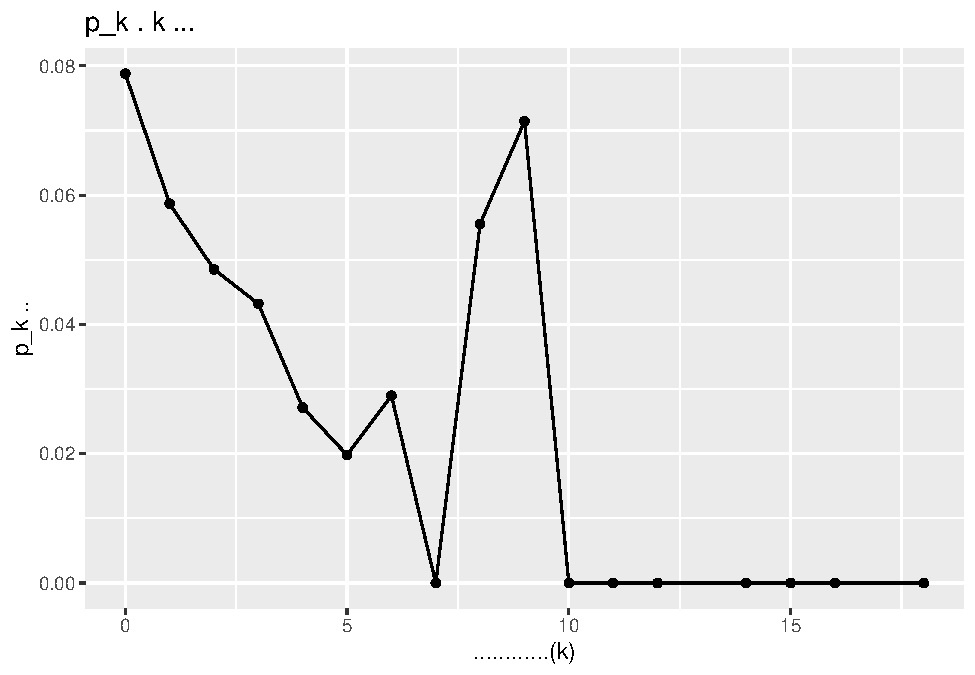
\includegraphics[keepaspectratio]{homework4_files/figure-latex/unnamed-chunk-5-1.pdf}}

\subsubsection{c}\label{c}

\begin{Shaded}
\begin{Highlighting}[]
\NormalTok{q\_k\_df }\OtherTok{\textless{}{-}}\NormalTok{ result\_df }\SpecialCharTok{\%\textgreater{}\%} 
  \FunctionTok{filter}\NormalTok{(started\_this\_month }\SpecialCharTok{==} \ConstantTok{TRUE}\NormalTok{) }\SpecialCharTok{\%\textgreater{}\%} 
  \FunctionTok{group\_by}\NormalTok{(contacts\_started\_by) }\SpecialCharTok{\%\textgreater{}\%} 
  \FunctionTok{summarise}\NormalTok{(}
    \AttributeTok{total =} \FunctionTok{nrow}\NormalTok{(}\FunctionTok{filter}\NormalTok{(result\_df, contacts\_started\_by }\SpecialCharTok{==} \FunctionTok{cur\_group\_id}\NormalTok{())),}
    \AttributeTok{success =} \FunctionTok{sum}\NormalTok{(started\_this\_month),}
    \AttributeTok{q\_k =}\NormalTok{ success }\SpecialCharTok{/}\NormalTok{ total}
\NormalTok{  )}


\FunctionTok{ggplot}\NormalTok{(q\_k\_df, }\FunctionTok{aes}\NormalTok{(}\AttributeTok{x =}\NormalTok{ contacts\_started\_by, }\AttributeTok{y =}\NormalTok{ q\_k)) }\SpecialCharTok{+} 
  \FunctionTok{geom\_point}\NormalTok{() }\SpecialCharTok{+} \FunctionTok{geom\_line}\NormalTok{() }\SpecialCharTok{+} 
  \FunctionTok{labs}\NormalTok{(}\AttributeTok{x =} \StringTok{"当月及之前已采用的联系人数量(k)"}\NormalTok{, }\AttributeTok{y =} \StringTok{"q\_k 概率"}\NormalTok{, }\AttributeTok{title =} \StringTok{"q\_k 与 k 的关系"}\NormalTok{)}
\end{Highlighting}
\end{Shaded}

\pandocbounded{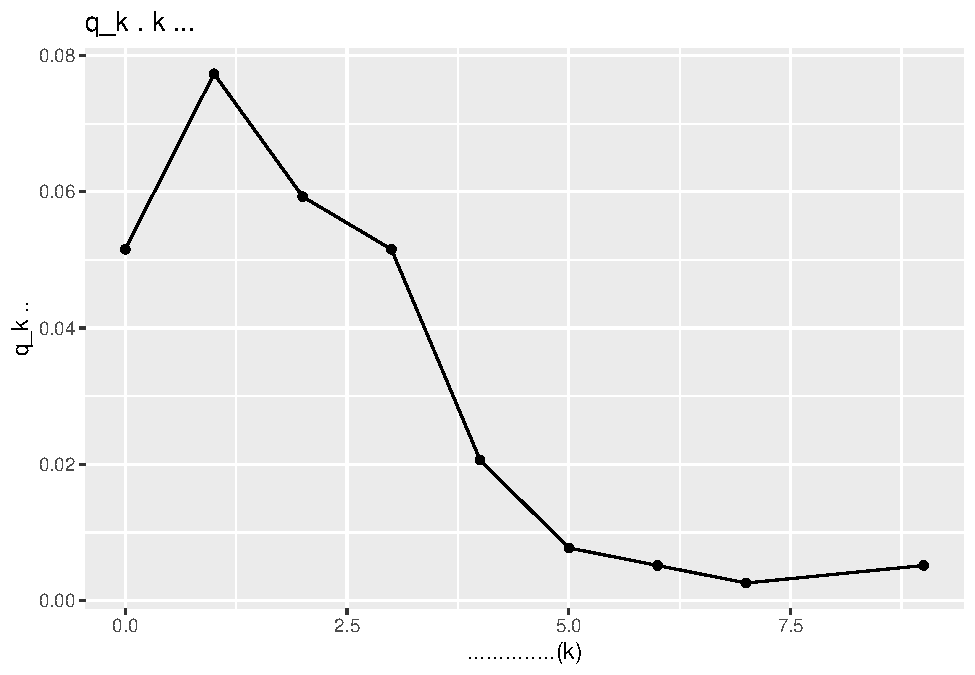
\includegraphics[keepaspectratio]{homework4_files/figure-latex/unnamed-chunk-6-1.pdf}}

\subsection{4}\label{section-3}

\subsubsection{a}\label{a-1}

\begin{Shaded}
\begin{Highlighting}[]
\CommentTok{\# 基于 3.b 得到的 p\_k\_df,拟合线性模型}
\NormalTok{linear\_fit }\OtherTok{\textless{}{-}} \FunctionTok{lm}\NormalTok{(p\_k }\SpecialCharTok{\textasciitilde{}}\NormalTok{ contacts\_started\_before, }\AttributeTok{data =}\NormalTok{ p\_k\_df)}


\NormalTok{a\_linear }\OtherTok{\textless{}{-}} \FunctionTok{coef}\NormalTok{(linear\_fit)[}\DecValTok{1}\NormalTok{] }
\NormalTok{b\_linear }\OtherTok{\textless{}{-}} \FunctionTok{coef}\NormalTok{(linear\_fit)[}\DecValTok{2}\NormalTok{]  }


\FunctionTok{ggplot}\NormalTok{(p\_k\_df, }\FunctionTok{aes}\NormalTok{(}\AttributeTok{x =}\NormalTok{ contacts\_started\_before, }\AttributeTok{y =}\NormalTok{ p\_k)) }\SpecialCharTok{+} 
  \FunctionTok{geom\_point}\NormalTok{() }\SpecialCharTok{+} 
  \FunctionTok{geom\_abline}\NormalTok{(}\AttributeTok{intercept =}\NormalTok{ a\_linear, }\AttributeTok{slope =}\NormalTok{ b\_linear, }\AttributeTok{color =} \StringTok{"red"}\NormalTok{, }\AttributeTok{linetype =} \StringTok{"dashed"}\NormalTok{) }\SpecialCharTok{+} 
  \FunctionTok{labs}\NormalTok{(}\AttributeTok{title =} \StringTok{"线性模型拟合:p\_k = a + bk"}\NormalTok{)}
\end{Highlighting}
\end{Shaded}

\pandocbounded{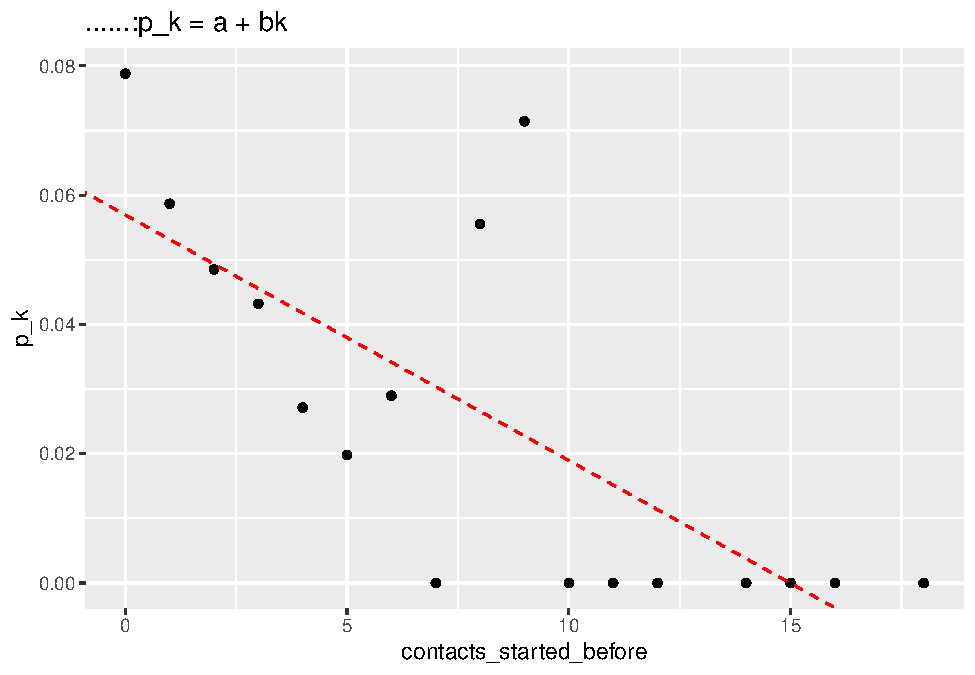
\includegraphics[keepaspectratio]{homework4_files/figure-latex/unnamed-chunk-7-1.pdf}}

\subsubsection{b}\label{b-1}

\begin{Shaded}
\begin{Highlighting}[]
\NormalTok{logistic\_model }\OtherTok{\textless{}{-}} \ControlFlowTok{function}\NormalTok{(k, a, b) \{}
  \FunctionTok{exp}\NormalTok{(a }\SpecialCharTok{+}\NormalTok{ b }\SpecialCharTok{*}\NormalTok{ k) }\SpecialCharTok{/}\NormalTok{ (}\DecValTok{1} \SpecialCharTok{+} \FunctionTok{exp}\NormalTok{(a }\SpecialCharTok{+}\NormalTok{ b }\SpecialCharTok{*}\NormalTok{ k))}
\NormalTok{\}}


\NormalTok{nonlinear\_fit }\OtherTok{\textless{}{-}} \FunctionTok{nls}\NormalTok{(}
\NormalTok{  p\_k }\SpecialCharTok{\textasciitilde{}} \FunctionTok{logistic\_model}\NormalTok{(contacts\_started\_before, a, b), }
  \AttributeTok{data =}\NormalTok{ p\_k\_df, }
  \AttributeTok{start =} \FunctionTok{list}\NormalTok{(}\AttributeTok{a =}\NormalTok{ a\_linear, }\AttributeTok{b =}\NormalTok{ b\_linear)  }\CommentTok{\# 用线性模型结果做初始值}
\NormalTok{)}


\FunctionTok{summary}\NormalTok{(nonlinear\_fit)}
\end{Highlighting}
\end{Shaded}

\begin{verbatim}
## 
## Formula: p_k ~ logistic_model(contacts_started_before, a, b)
## 
## Parameters:
##   Estimate Std. Error t value Pr(>|t|)    
## a -2.56508    0.20610 -12.446 2.62e-09 ***
## b -0.17051    0.05371  -3.174  0.00628 ** 
## ---
## Signif. codes:  0 '***' 0.001 '**' 0.01 '*' 0.05 '.' 0.1 ' ' 1
## 
## Residual standard error: 0.01957 on 15 degrees of freedom
## 
## Number of iterations to convergence: 7 
## Achieved convergence tolerance: 1.592e-07
\end{verbatim}

\begin{Shaded}
\begin{Highlighting}[]
\NormalTok{a\_logistic }\OtherTok{\textless{}{-}} \FunctionTok{coef}\NormalTok{(nonlinear\_fit)[}\StringTok{"a"}\NormalTok{]}
\NormalTok{b\_logistic }\OtherTok{\textless{}{-}} \FunctionTok{coef}\NormalTok{(nonlinear\_fit)[}\StringTok{"b"}\NormalTok{]}


\NormalTok{k\_range }\OtherTok{\textless{}{-}} \FunctionTok{seq}\NormalTok{(}\FunctionTok{min}\NormalTok{(p\_k\_df}\SpecialCharTok{$}\NormalTok{contacts\_started\_before), }\FunctionTok{max}\NormalTok{(p\_k\_df}\SpecialCharTok{$}\NormalTok{contacts\_started\_before), }\AttributeTok{by =} \DecValTok{1}\NormalTok{)}
\NormalTok{predicted }\OtherTok{\textless{}{-}} \FunctionTok{logistic\_model}\NormalTok{(k\_range, a\_logistic, b\_logistic)}

\FunctionTok{ggplot}\NormalTok{(p\_k\_df, }\FunctionTok{aes}\NormalTok{(}\AttributeTok{x =}\NormalTok{ contacts\_started\_before, }\AttributeTok{y =}\NormalTok{ p\_k)) }\SpecialCharTok{+} 
  \FunctionTok{geom\_point}\NormalTok{() }\SpecialCharTok{+} 
  \FunctionTok{geom\_line}\NormalTok{(}\AttributeTok{data =} \FunctionTok{data.frame}\NormalTok{(}\AttributeTok{k =}\NormalTok{ k\_range, }\AttributeTok{p =}\NormalTok{ predicted), }
            \FunctionTok{aes}\NormalTok{(}\AttributeTok{x =}\NormalTok{ k, }\AttributeTok{y =}\NormalTok{ p), }\AttributeTok{color =} \StringTok{"blue"}\NormalTok{, }\AttributeTok{linetype =} \StringTok{"dashed"}\NormalTok{) }\SpecialCharTok{+} 
  \FunctionTok{labs}\NormalTok{(}\AttributeTok{title =} \StringTok{"非线性模型拟合:p\_k = e\^{}(a+bk)/(1+e\^{}(a+bk))"}\NormalTok{)}
\end{Highlighting}
\end{Shaded}

\pandocbounded{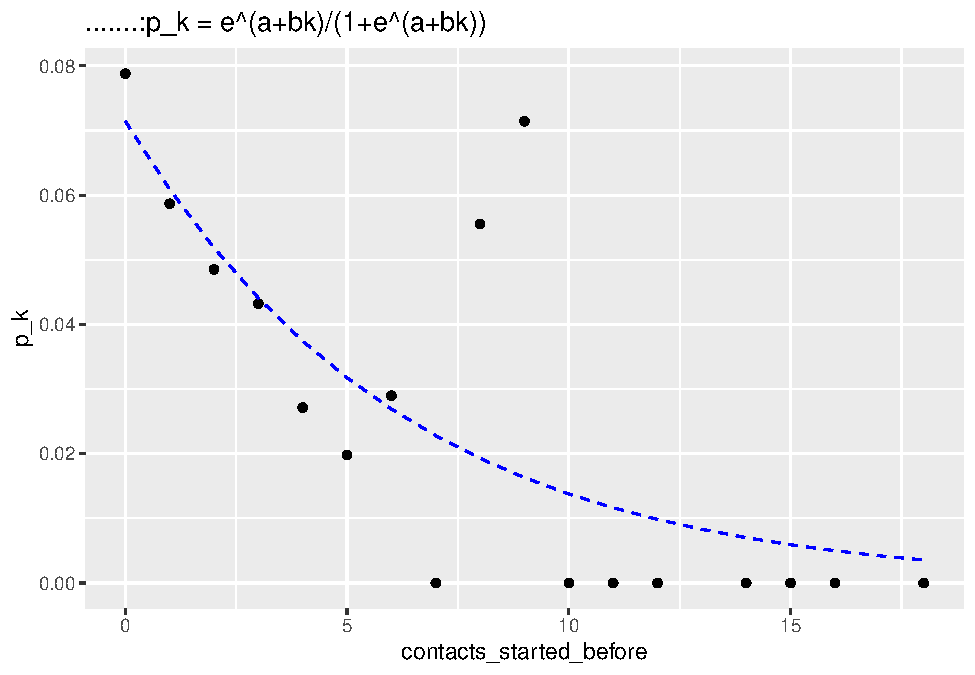
\includegraphics[keepaspectratio]{homework4_files/figure-latex/unnamed-chunk-8-1.pdf}}

\subsubsection{c}\label{c-1}

\begin{Shaded}
\begin{Highlighting}[]
\NormalTok{pred\_linear }\OtherTok{\textless{}{-}}\NormalTok{ a\_linear }\SpecialCharTok{+}\NormalTok{ b\_linear }\SpecialCharTok{*}\NormalTok{ k\_range}
\NormalTok{pred\_logistic }\OtherTok{\textless{}{-}} \FunctionTok{logistic\_model}\NormalTok{(k\_range, a\_logistic, b\_logistic)}


\FunctionTok{ggplot}\NormalTok{(p\_k\_df, }\FunctionTok{aes}\NormalTok{(}\AttributeTok{x =}\NormalTok{ contacts\_started\_before, }\AttributeTok{y =}\NormalTok{ p\_k)) }\SpecialCharTok{+} 
  \FunctionTok{geom\_point}\NormalTok{(}\AttributeTok{color =} \StringTok{"black"}\NormalTok{) }\SpecialCharTok{+} 
  \FunctionTok{geom\_line}\NormalTok{(}\AttributeTok{data =} \FunctionTok{data.frame}\NormalTok{(}\AttributeTok{k =}\NormalTok{ k\_range, }\AttributeTok{p =}\NormalTok{ pred\_linear), }
            \FunctionTok{aes}\NormalTok{(}\AttributeTok{x =}\NormalTok{ k, }\AttributeTok{y =}\NormalTok{ p), }\AttributeTok{color =} \StringTok{"red"}\NormalTok{, }\AttributeTok{linetype =} \StringTok{"dashed"}\NormalTok{, }\AttributeTok{size =} \DecValTok{1}\NormalTok{) }\SpecialCharTok{+} 
  \FunctionTok{geom\_line}\NormalTok{(}\AttributeTok{data =} \FunctionTok{data.frame}\NormalTok{(}\AttributeTok{k =}\NormalTok{ k\_range, }\AttributeTok{p =}\NormalTok{ pred\_logistic), }
            \FunctionTok{aes}\NormalTok{(}\AttributeTok{x =}\NormalTok{ k, }\AttributeTok{y =}\NormalTok{ p), }\AttributeTok{color =} \StringTok{"blue"}\NormalTok{, }\AttributeTok{linetype =} \StringTok{"dashed"}\NormalTok{, }\AttributeTok{size =} \DecValTok{1}\NormalTok{) }\SpecialCharTok{+} 
  \FunctionTok{labs}\NormalTok{(}
    \AttributeTok{x =} \StringTok{"联系人数量(k)"}\NormalTok{, }
    \AttributeTok{y =} \StringTok{"采用概率(p\_k)"}\NormalTok{, }
    \AttributeTok{title =} \StringTok{"线性 vs 非线性模型拟合对比"}\NormalTok{,}
    \AttributeTok{caption =} \StringTok{"红色:线性模型;蓝色:逻辑斯蒂模型"}
\NormalTok{  )}
\end{Highlighting}
\end{Shaded}

\begin{verbatim}
## Warning: Using `size` aesthetic for lines was deprecated in ggplot2 3.4.0.
## i Please use `linewidth` instead.
## This warning is displayed once every 8 hours.
## Call `lifecycle::last_lifecycle_warnings()` to see where this warning was
## generated.
\end{verbatim}

\pandocbounded{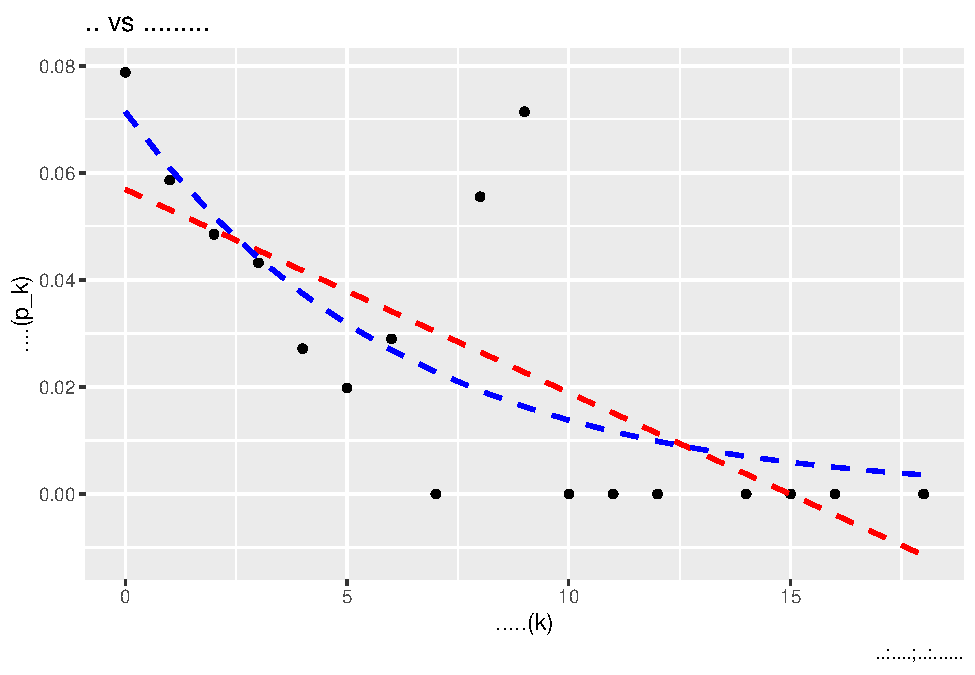
\includegraphics[keepaspectratio]{homework4_files/figure-latex/unnamed-chunk-9-1.pdf}}

\end{document}
